\documentclass[a4paper,12pt]{report}

\usepackage[pdftex]{graphicx}
\DeclareGraphicsExtensions{.pdf}
\usepackage{amsmath}
\usepackage{amssymb}

% Title Page
\title{Test Report on Kinetic Energy Density Implementation in Norm-Conserving Plane-Waves Formalism.}
\author{Aur\'{e}lien Lherbier}


\begin{document}
\maketitle

\chapter{Test on an isolated H atom.}
\label{chapter1}

We use the Fermi-Amaldi exchange-correlation functional ($ixc=20$) and no spin polarization (not available with this functional).\\
For single H atom we have the wavefunction which is $1s$ atomic orbital.
For analytical approach\footnote{For theoritical and implementation details see chap. $2$ in /doc/theory/ELF/} we thus use the spherical harmonic formulation which is given by:

\begin{equation}
\psi = \varphi_{1s}(r,\theta,\phi) = \sqrt{\frac{Z^3}{\pi a_0^3}} e^{-Z \frac{\vert \mathbf{r} \vert}{a_0}}
\end{equation}

with $Z$ the atomic number and $a_0$ the Bohr constant.\\
We obtain for H atom ($Z=1$):\\

\begin{itemize}
\item the electronic density
\begin{equation}
\vert \psi \vert^2 = \vert \varphi_{1s}(r,\theta,\phi) \vert^2 = \frac{1}{\pi a_0^3} e^{-\frac{2\vert \mathbf{r} \vert}{a_0}}
\end{equation}
\item the kinetic energy density
\begin{equation}
\frac{1}{2} \vert \nabla \psi \vert^2 = \frac{1}{2} \vert \nabla \varphi_{1s}(r,\theta,\phi) \vert^2 = \frac{1}{2\pi a_0^5} e^{-\frac{2\vert \mathbf{r} \vert}{a_0}}
\end{equation}
\end{itemize}

We work in Bohr unit, $a_0=1$, hence we have the same form, up to a factor $\frac{1}{2}$, for electronic density and kinetic energy density for the isolated H atom ($\frac{1}{\pi} e^{-2\vert \mathbf{r} \vert}$) but in different units (Bohr$^{-3}$ and Bohr$^{-5}$). In the following we miss the factor $\frac{1}{2}$ in the kinetic energy density for comparison.\\\\\\

\section{Standard test.}
\label{section1}
The standard input file used is the following:\\
acell 3*30\\
ecut 250\\
diemac 1.0d0\\
diemix 0.5d0\\
iscf 3\\
ixc 20\\
kpt 3*0.25\\
natom 1\\
nband 1\\
nkpt 1\\
nline 3\\
nsppol 1\\
nstep 6\\
nsym 8\\
ntypat 1\\
occ 1\\
rprim 100 010 001\\
symrel\\
 1 0 0\hspace{0.3cm}   0 1 0\hspace{0.3cm}   0 0 1\\
-1 0 0\hspace{0.3cm}   0 1 0\hspace{0.3cm}   0 0 1\\
 1 0 0\hspace{0.3cm}   0-1 0\hspace{0.3cm}   0 0 1\\
-1 0 0\hspace{0.3cm}   0-1 0\hspace{0.3cm}   0 0 1\\
 1 0 0\hspace{0.3cm}   0 1 0\hspace{0.3cm}   0 0-1\\
-1 0 0\hspace{0.3cm}   0 1 0\hspace{0.3cm}   0 0-1\\
 1 0 0\hspace{0.3cm}   0-1 0\hspace{0.3cm}   0 0-1\\
-1 0 0\hspace{0.3cm}   0-1 0\hspace{0.3cm}   0 0-1\\
tnons 24*0\\
tolwfr 1.0d-14\\
typat 1\\
wtk 1\\
znucl 1\\
xred 3*0\\
prtkden 1  \#output a  \_KDEN file.\\\\\\\\\\

We observe on the following picture (Fig.(\ref{fig1})) the result of ABINIT compared to previous analytical formula.\\
The ABINIT rhor and taur are respectively electron density and kinetic energy density along the x-axis (100) and passing through H atom (being at (0,0,0)).
We see that for electron density we found a good agreement. This is only very close to the H atom that ABINIT rhor start to be underestimated.\\
However for ABINIT taur, there is a discrepancy within the region very close to the H atom (the rest is correct). Indeed ABINIT taur goes to 0 at the exact H position.
However it seems  to be consistent with the fact that the 1rst derivative of the ABINIT wavefunction at exact H position is 0. This is also why electron density is underestimated compared to analytical curves.

\begin{figure}[!h]
\centering
\begin{minipage}[c]{1.0\textwidth}
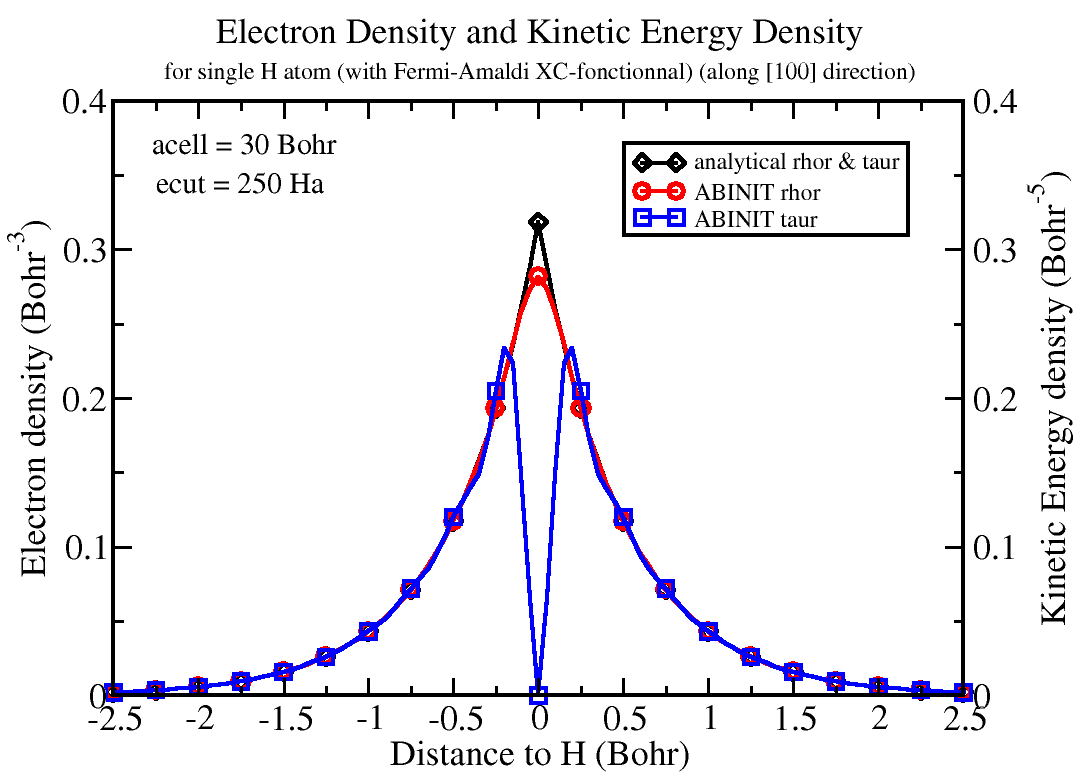
\includegraphics[width = \textwidth]{fig1}
\end{minipage}
\vspace{0.12\textwidth}
\begin{minipage}[c]{0.8\textwidth}
\caption{\small Comparison between analytical densities and ABINIT densities for a isolated H atom.}
\vspace*{1.0ex}
\label{fig1}
\end{minipage}
\end{figure}

\section{More tests.}
\label{section2}
In previous page we did not care about convergence. Here we look first at the convergence study with the size of the box (acell convergence study), and then with kinetic energy cut-off (ecut convergence study).

\begin{figure}[!h]
\centering
\begin{minipage}[c]{0.7\textwidth}
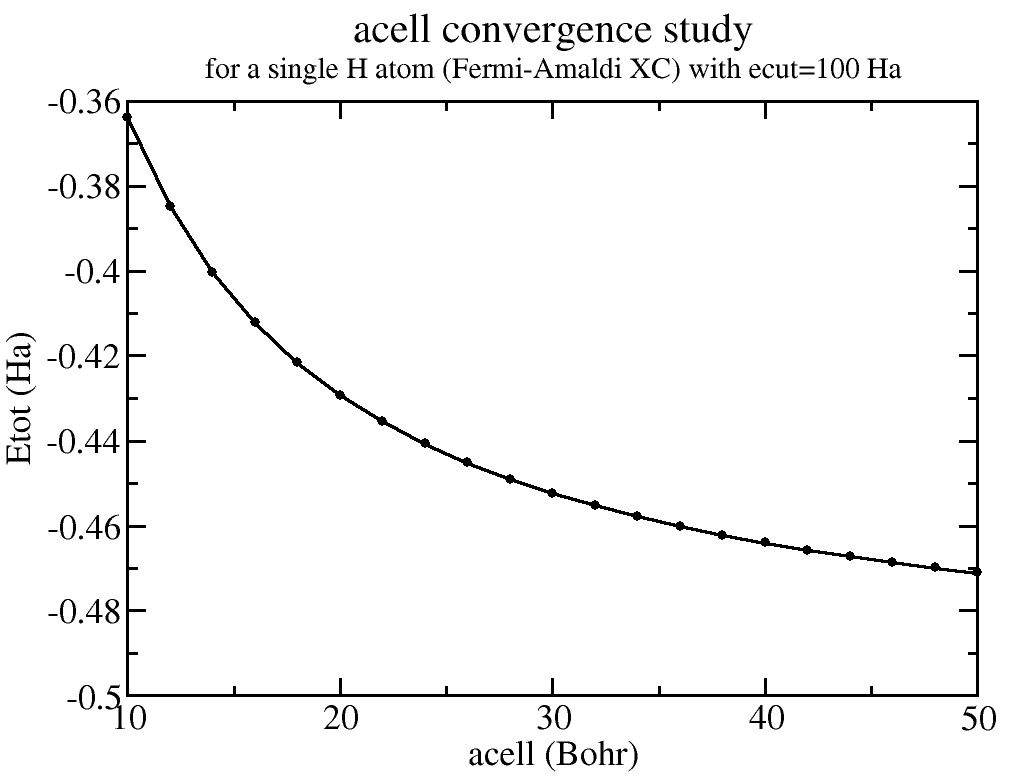
\includegraphics[width = \textwidth]{acell_fixecut_convergence_crop}
\end{minipage}
\vspace{0.12\textwidth}
\begin{minipage}[c]{0.7\textwidth}
\caption{\small Total energy vs acell.}
\vspace*{1.0ex}
\label{etot_acell}
\end{minipage}
\end{figure}

\begin{figure}[!h]
\centering
\begin{minipage}[c]{0.7\textwidth}
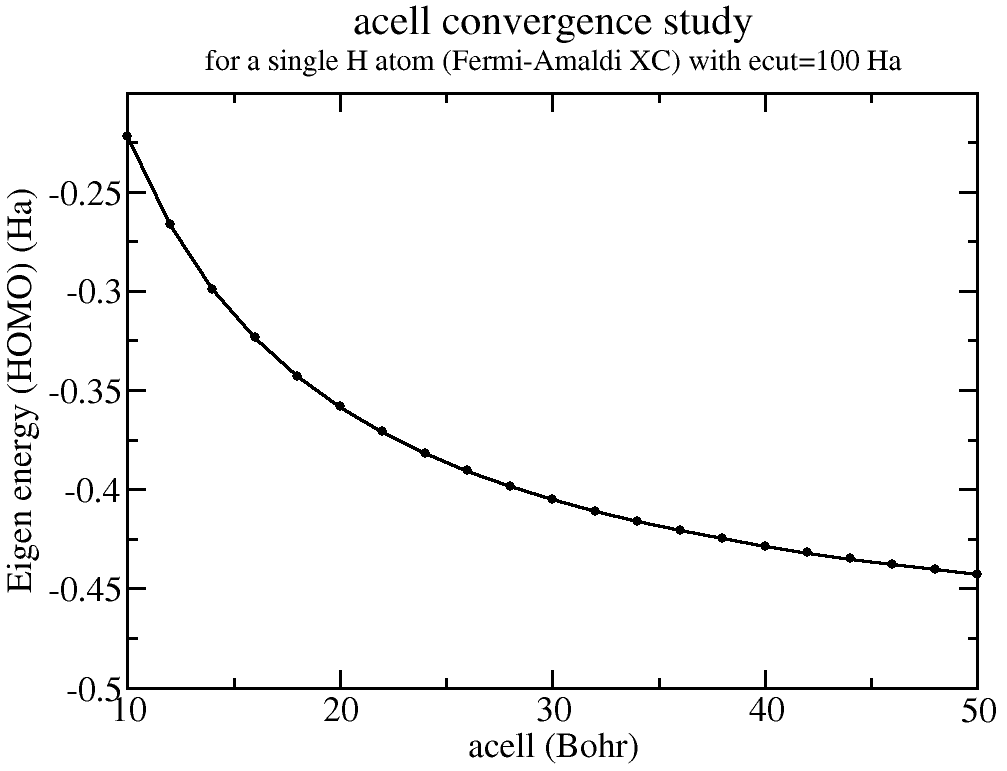
\includegraphics[width = \textwidth]{eigval_vs_acell_crop}
\end{minipage}
\vspace{0.12\textwidth}
\begin{minipage}[c]{0.7\textwidth}
\caption{\small Eigen energy vs acell.}
\vspace*{1.0ex}
\label{eig_acell}
\end{minipage}
\end{figure}

\begin{figure}[!h]
\centering
\begin{minipage}[c]{1.0\textwidth}
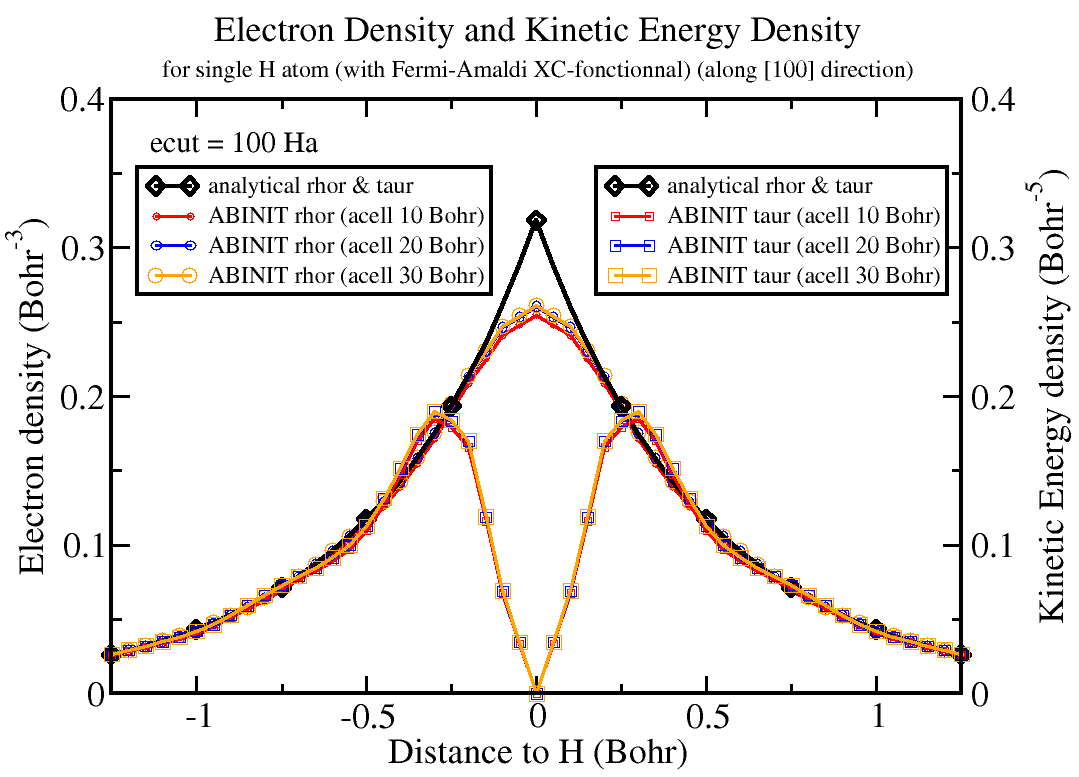
\includegraphics[width = \textwidth]{H_DEN_KDEN_line100_acell_crop}
\end{minipage}
\vspace{0.12\textwidth}
\begin{minipage}[c]{0.7\textwidth}
\caption{\small electron density and kinetic energy density vs acell.}
\vspace*{1.0ex}
\label{den_kden_acell}
\end{minipage}
\end{figure}

\begin{figure}[!h]
\centering
\begin{minipage}[c]{0.7\textwidth}
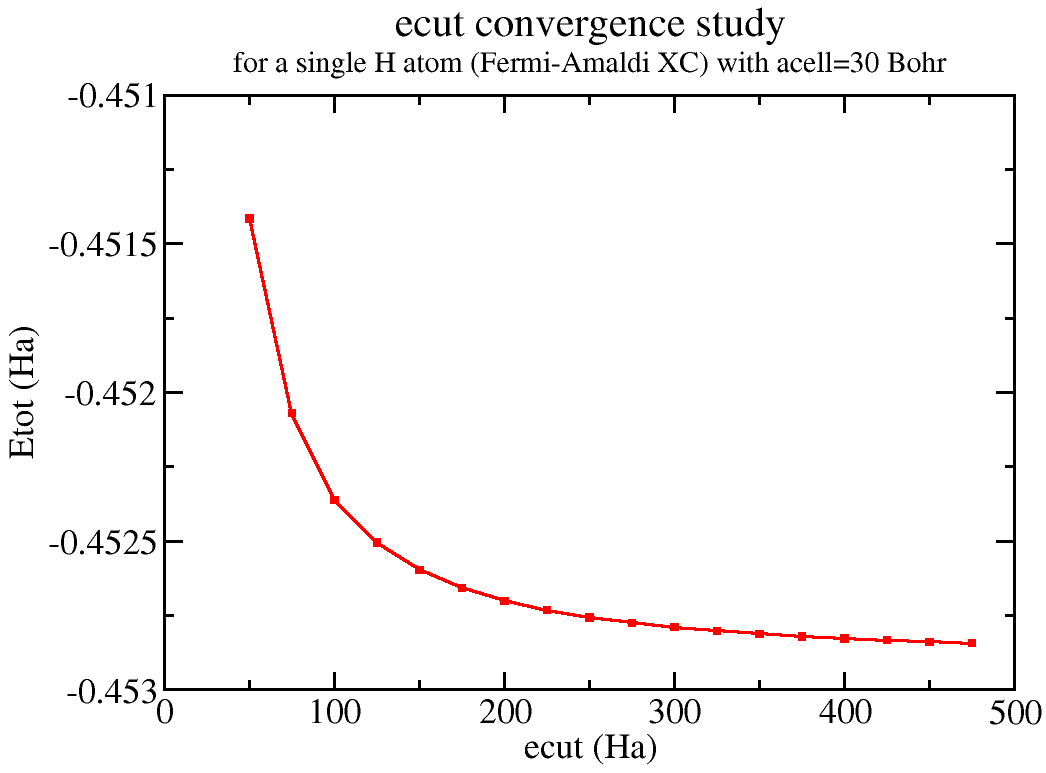
\includegraphics[width = \textwidth]{ecut_fixacell_convergence_crop}
\end{minipage}
\vspace{0.12\textwidth}
\begin{minipage}[c]{0.7\textwidth}
\caption{\small Total energy vs ecut.}
\vspace*{1.0ex}
\label{etot_ecut}
\end{minipage}
\end{figure}

\begin{figure}[!h]
\centering
\begin{minipage}[c]{0.7\textwidth}
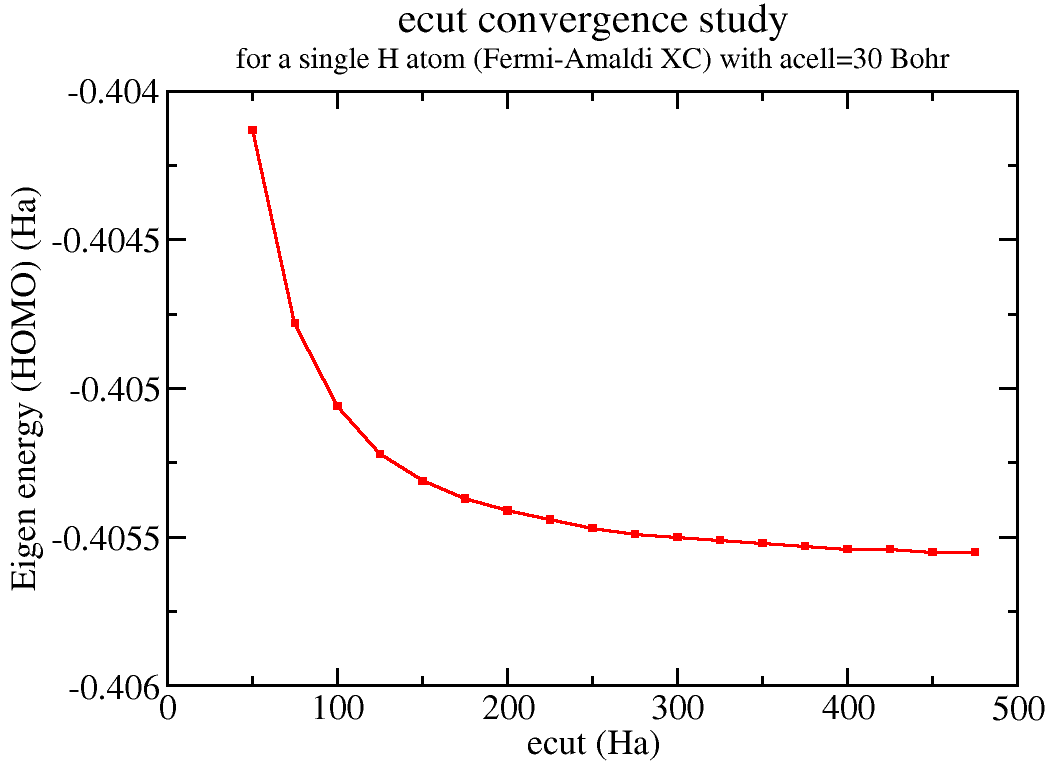
\includegraphics[width = \textwidth]{eigval_vs_ecut_crop}
\end{minipage}
\vspace{0.12\textwidth}
\begin{minipage}[c]{0.7\textwidth}
\caption{\small Eigen energy vs ecut.}
\vspace*{1.0ex}
\label{eig_ecut}
\end{minipage}
\end{figure}

\begin{figure}[!h]
\centering
\begin{minipage}[c]{1.0\textwidth}
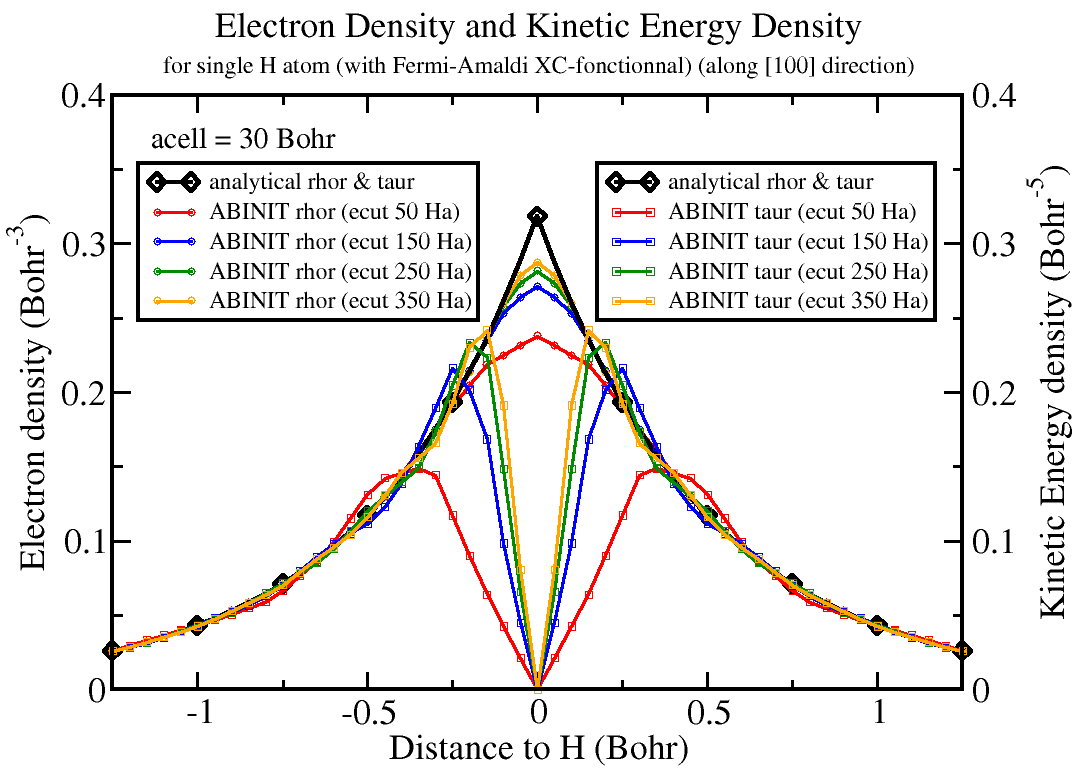
\includegraphics[width = \textwidth]{H_DEN_KDEN_line100_ecut_crop}
\end{minipage}
\vspace{0.12\textwidth}
\begin{minipage}[c]{0.7\textwidth}
\caption{\small electron density and kinetic energy density vs ecut.}
\vspace*{1.0ex}
\label{den_kden_ecut}
\end{minipage}
\end{figure}

\section{Additional tests.}
We have checked also that the implementation for spin polarized system works. For instance we have tried isolated Bismuth (Bi) atom. We have used for that the already existing test \textit{v5/t31.in} in which we have added \textit{prtkden 1}.\\
We have also tested the parallel implementation (abinip) with 1-2-4 processors and have checked that the result is the same than in sequential version (abinis).



\end{document}
